\documentclass[../main.tex]{subfiles}
\begin{document}
\lstset{language=Matlab}
\section*{Introduction}
Our goal in this assignment is to code linear and quadratic
\textit{isoparametric} triagular finite elements.In finite element
analysis, both the geometry and the unknown solution field are
discretized using suitable interpolating functions. The term
\textit{parametric} indicates that we will develop shape functions for
a standard parametric domain. Using suitable Jacobian matrix we will
map these shape functions to the actual domain of integration. The
term \textit{iso} indicates that we will use the same shape functions
for both the geometrical domain and the unknown solution field. To
develop a numerical scheme for isoparametric triangular elements
requires triangular shape functions and quadrature scheme for
integration on triangular domains. These are the topics of the
succeeding sections.

\section*{Triangular Shape Functions}
We plan to develop shape functions for a linear 3-node triangular
element and quadratic 6-node triangular element. The standard
parametric triangular domains along with the nodes and their
parametric coordinates for these elements are shown in figures
~\ref{fig:linDom} and ~\ref{fig:quadDom}. The next two subsections
give the equations for shape functions and their derivatives for the
two cases.
\subsection*{Linear 3-node Triangular Shape Functions and Their
  Derivatives}
\begin{figure}[h]
  \centering
  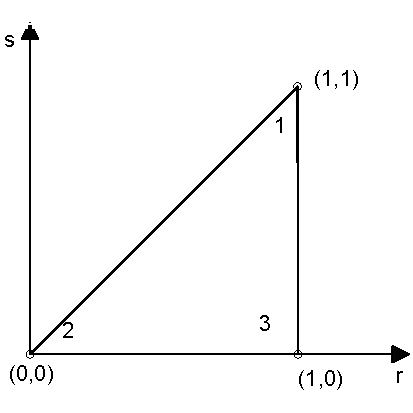
\includegraphics[scale=1]{./img/linearDomain.pdf}
  \caption{Nodal positions and numbering for linear parametric
    triangular domain}
  \label{fig:linDom}
\end{figure}
For three nodes we need three shape functions that satisfy the
Kronecker-Delta property. Barycentric co-ordinates for triangles
naturally satisfy this requirement. Hence the shape functions in terms
of the barycentric co-ordinates are
\begin{align*}
  \hat{N}_i = \lambda_i
\end{align*}
For the node numbering shown in the standard $(r,s)$ parametric domain
of Figure ~\ref{fig:linDom}, the barycentric coordinates, and thus the
shape functions, are given by
\begin{align}
  \label{eq:bary}
  \lambda_1 = s \qquad \lambda_2 = 1-r \qquad \lambda_3 = r-s
\end{align}
The derivatives are
\begin{alignat*}{3}
  \hat{N}_{1,r} &= 0 &\quad\hat{N}_{1,s} &= 1 \\
  \hat{N}_{2,r} &= -1& \quad\hat{N}_{2,s}&= 0 \\
  \hat{N}_{3,r} &= 1 & \quad\hat{N}_{3,s}&= -1
\end{alignat*}
\subsection*{Quadratic 6-node Triangular Shape Functions and Their
  Derivatives}
\begin{figure}[h]
  \centering
  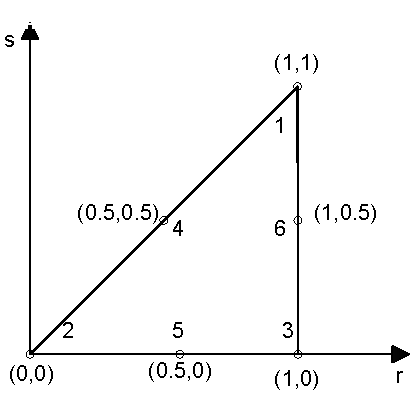
\includegraphics[scale=1]{./img/quadraticDomain.pdf}
  \caption{Node numbering and locations for quadratic parametric
    triangular domain}
  \label{fig:quadDom}
\end{figure}
The node numbering is shown in Figure ~\ref{fig:quadDom}. As the node
numbers $1,2$ and $3$ are same as for the linear 3-node case, we can
use the same barycentric coordinates as in Equation
~\ref{eq:bary}. The six shape functions in terms of the barycentric
coordinates are
\begin{center}
  \begin{alignat*}{2}
    \hat{N}_1 &= \lambda_1(2\lambda_1-1) &&= -s+2s^2 \\
    \hat{N}_2 &= \lambda_2(2\lambda_2-1) &&= 2r^2-3r+1\\
    \hat{N}_3 &= \lambda_3(2\lambda_3-1) &&= 2r^2-r-4rs+s+2s^2\\
    \hat{N}_4 &= 4\lambda_1\lambda_2 &&= -4rs +4s \\
    \hat{N}_5 &= 4\lambda_2\lambda_3 &&=  -4(r^2-r-rs+s)\\
    \hat{N}_6 &= 4\lambda_3\lambda_1 &&= 4rs-4s^2
  \end{alignat*}
\end{center}
The derivatives are
\begin{alignat*}{3}
  \hat{N}_{1,r} &= 0 &\quad\hat{N}_{1,s} &= 4s-1 \\
  \hat{N}_{2,r} &= 4r-3 &\quad\hat{N}_{2,s}&= 0 \\
  \hat{N}_{3,r} &= 4r-4s-1&\quad\hat{N}_{3,s} &= 1-4r+4s \\
  \hat{N}_{4,r} &= -4s &\quad\hat{N}_{4,s} &= 4(1-r) \\
  \hat{N}_{5,r} &= 4(1-2r+s)&\quad\hat{N}_{5,s} &= 4(r-1) \\
  \hat{N}_{6,r} &= 4s&\quad\hat{N}_{6,s} &= 4(r-2s)
\end{alignat*}

\section*{Gaussian Quadrature on Triangular Domain}
The equations for elastic response of isoparametric triangular
elements have integrals evaluated over a triangular domain of
integration. We will use Gaussian Quadrature rules for numerical
integration. For the standard parametric domain of Figure
~\ref{fig:linDom} the general form of Gaussian quadrature is
\begin{align*}
  \int^1_0\int^r_0\!f(r,s)\,\mathrm{d}s\mathrm{d}r = \sum^{n_G}_{i=1}\hat{w}_if(r_i,s_i)\hat{\Omega}
\end{align*}
where $n_G$ is the number of sampling points $(r_i,s_i)$ and
$\hat{w}_i$ is the corresponding weight normalized by the area of the
domain $\hat{\Omega}=(1/2)$.  Table ~\ref{tab:gaussQuad} gives the
values of $n_G$, $\hat{w}_i$ and $(r_i,s_i)$ for the 1-point and
3-point quadrature.
\begin{table}
  \centering
  \caption{Sampling points and weights for 1-point and 3-point Gaussian quadrature}\label{tab:gaussQuad}
  \begin{tabular}{|>{$}c<{$}|>{$}c<{$}|>{$}c<{$}|}
    \hline
    n_G & \hat{w}_i & (r_i,s_i) \\[5pt]
    \hline
    1 & w_1 = 1 & (2/3,1/3) \\[5pt]
    \hline
        & w_1 = (1/3) & (1/2,1/2) \\
    3 & w_2 = (1/3) & (1,1/2) \\
        & w_3 = (1/3) & (1/2,0) \\
    \hline
  \end{tabular}  
\end{table}

\section*{Isoparametric Triangular Elements}
Using either of the shape functions and one of the quadrature rules
discussed in previous sections we can write the equations for strain
energy, internal force and stiffness modulus of isoparametric
triangular elements.  Let $\mathbf{X}$ and $\mathbf{x}$ represent the
reference and deformed configurations of the element. Also, we will
denote the parametric domain as $\theta^\alpha$ where $\theta^1 = r$
and $\theta^2=s$. Let $n$ be the number of nodes in the element. In
all the following equations $i,J,k,L,\alpha,\beta = 1,2$ and
$a=1,2\ldots n$. The Jacobian matrix for transformation from
parametric domain to reference configuration is then given as
\begin{align*}
  \mathbb{J}_{I\alpha} = \frac{\partial X_{I}}{\partial\theta^{\alpha}}
\end{align*}
The derivative of the shape functions with respect to $\mathbf{X}$ are
\begin{align*}
  N_{a,J} &= \frac{\partial N_a}{\partial X_{aJ}}\\
          &= \frac{\partial\hat{N}_a}{\partial\theta_{\beta}}\frac{\partial\theta_{\beta}}{\partial X_{J}}\\
          &= \hat{N}_{a,\beta}\mathbb{J}^{-1}_{\beta J}
\end{align*}
The deformation gradient can now be written as
\begin{align*}
  F_{iJ} = x_{ia}N_{a,J}
\end{align*}
It is important that the sequence of vertices of the triangular domain
$\mathbf{X}$ and $\mathbf{x}$ must be same as formed by the node
numbering of the standard domain in Figures ~\ref{fig:linDom} and
~\ref{fig:quadDom}. If this requirement is not met, the determinant of
$\mathbf{F}$ will become negative and give rise to imaginary
Piola-Kirchhoff stress tensor. Also, the triangles should not have
very high asspect ratio as that can cause determinant of $\mathbf{F}$
approach $0$ and cause problems in calculating $\mathbf{F}^{-1}$.

Once we have a valid deformation gradient we can calculate the strain
energy density $w$, the Piola-Kirchhoff stress tensor $P_{iJ}$ and the
consistent two-dimensional stiffness tensor $C_{iJkL}$ using the plane
stress neo-Hookean constitutive relationship formulated in HW 1.  We
need the following integral equations to find strain energy $W$, the
internal force $f^{\text{int}}_{ia}$ and the stiffness modulus
$K_{iakb}$ for the element $\Omega^e$
\begin{align*}
  W &=\int_{\Omega^e}\!w\,\mathrm{d}\Omega^e\\[5pt]
    &=\sum_{q=1}^{n_G}w\bigg\lvert_{\theta_q}\hat{w}_q\lvert\mathbb{J}\lvert\hat{\Omega}
\end{align*}
\begin{align*}
  f_{ia}^{\text{int}} &= \int_{\Omega^e}\!P_{iJ}N_{a,J}\,\mathrm{d}\Omega^e\\[5pt]
                      &=\sum_{q=1}^{n_G}\left(P_{iJ}\hat{N}_{a,\beta}\mathbb{J}^{-1}_{\beta J}\right)\bigg\lvert_{\theta_q}\hat{w}_q\lvert\mathbb{J}\lvert\hat{\Omega}
\end{align*}
\begin{align*}
  K_{iakb} &= \int_{\Omega^e}\!C_{iJkL}N_{a,J}N_{b,L}\,\mathrm{d}\Omega^e\\
           &=\sum_{q=1}^{n_G}\left(C_{iJkL}\hat{N}_{a,\beta}\mathbb{J}^{-1}_{\beta J}\hat{N}_{b,\alpha}\mathbb{J}^{-1}_{\alpha L}\right)\bigg\lvert_{\theta_q}\hat{w}_q\lvert\mathbb{J}\lvert\hat{\Omega}
\end{align*}
\section*{Verification Tests for Shape Functions, Quadrature and
  Elements}
To verify the correctness of our computer implementations, we will
check for some known properties that the shape functions, quadrature
and elements should satisfy.

\subsection*{Verification of Shape Functions}
\begin{itemize}
\item Partition of unity: At any point $(r_1,s_1)$ in the standard
  domain, the shape functions should have
  \begin{align*}
    \sum_{a=1}^n\hat{N}_a(r_1,s_1) = 1
  \end{align*}
  We generated 1000 random points in the domain and checked for this
  property for the linear 3-node and quadratic 6-node triangular shape
  functions. It was satisfied with a numberical tolerance of
  $1\times10^{-15}$ in all cases.
\item Partition of nullity: The shape function derivatives should
  satisfy
  \begin{align*}
    \sum_{a=1}^n\hat{N}_{a,\alpha}(r,s) = 0\qquad\alpha=1,2
  \end{align*} at all points in the standard
  domain. For 1000 randomly generated points in the domain this
  property was found to be satisfied with a numerical tolerance of
  $1\times10^{-15}$ for both the 3-node linear and 6-node quadratic 
  shape functions.
\item Consistency: The shape function derivatives calculated by our
  code should tally with finite difference approximations of the
  derivatives within a suitable numerical tolerance. To get finite
  difference approximation of derivative with respect to one of the
  coordiantes $r$ and $s$ we perturb that co-ordinate with a suitably
  small value while holding the other coordinate constant. For
  example, using central finite differences we can write
  \begin{align*}
    \hat{N}_{a,r} \approx \frac{\hat{N}_{a}(r+h,s) - \hat{N}_{a}(r-h,s)}{2h}
  \end{align*}
  where $h$ is the perturbation. The value of $h$ was chosen to be of
  the order $10^{-6}$. For values of $h$ smaller than this, large
  rounding errors make the approximation to have errors larger than
  $\mathcal{O}(h)$ . For both the 3-node linear and 6-node quadratic
  shape functions the derivatives calculated by our code tallied with
  the corresponding central finite difference approximations to an
  acceptable tolerance of $10^{-6}$.
\item $C^0$-completeness: For a finite element formulation to converge
  to a solution, one of the requirements is that the shape functions
  should be able to exactly reproduce a linear field. Irrespective of
  the actual functional form of the solution field over the full
  domain, if it is discretized over sufficiently small elements then
  the local form of the solution over the element can always be
  reasonably approximated using linear functions. This is the
  rationale behind $C^0$-completeness requirement. To test it we will
  use a linear polynomial in $(r,s)$, that is, $p(r,s) = ar+bs+c$ where
  $a,b$ and $c$ are randomly chosen co-efficients. We will evaluate
  $p$ at the nodes of the standard domain to get $p(r_a,s_a)$. For a
  randomly chosen point $(r_1,s_1)$ in the domain, $C^0$-completeness
  requires
  \begin{align*}
    p(r_1,s_1) = \sum_{a=1}^n\hat{N}_a(r_a,s_a)p(r_a,s_a)
  \end{align*}
  For both the 3-node linear and 6-node quadratic shape functions we
  found this to be true with an error of the order $10^{-14}$. The
  error is small enough to consider this verification test as passed.
\end{itemize}

\subsection*{Verification of Quadrature Implementation}
A Gaussian quadrature rule that uses $n$ points should exactly
reproduce integration of a polynomial of degree less than or equal to
$2n-1$. We have implemented 1-point and 3-point quadrature rules. But
our shape functions are only linear or quadratic. So we will check, if
our 1-point quadrature code can reproduce integration of a linear
polynomial in $(r,s)$ and if our 3-point quadrature code can reproduce
integration of a quadratic polynomial in $(r,s)$ exactly over the
standard domain of Figure ~\ref{fig:linDom}.
\begin{itemize}
\item For a linear polynomial,
  \begin{align*}
    I_1 &= \int_0^1\int_0^r\!(ar+bs+c)\,\mathrm{d}s\mathrm{d}r \\
        &= \frac{a}{3}+\frac{b}{6}+\frac{c}{2}
  \end{align*}
  For 1-point scheme the sampling point is $(r_1,s_1)=((2/3),(1/3))$
  and $\hat{w}_1 = 1$. Area of the standard domain is
  $\hat{\Omega} = (1/2)$. We want to check if our code returns
  \begin{align*}
    (ar_1+bs_1+c)\hat{w}_1\hat{\Omega} = I_1
  \end{align*}
  We found this to satisfied for each of 1000 random choices for $a,b$
  and $c$ with a tolerance of the order $10^{-15}$.
\item For a quadratic polynomial,
  \begin{align*}
    I_3 &= \int_0^1\int_0^r\!(ar^2+bs^2+crs+dr+es+f)\,\mathrm{d}s\mathrm{d}r \\
        &= \frac{1}{24}(6a+2b+3c+8d+4e+12f)
  \end{align*} 
  For 3-point scheme the sampling points and weights are given in
  Table ~\ref{tab:gaussQuad}. Area of the standard domain is
  $\hat{\Omega} = (1/2)$. We want to check if our code returns
  \begin{align*}
    \sum_{q=1}^3(ar^2_q+bs^2_q+cr_qs_q+dr_q+es_q+f)\hat{w}_q\hat{\Omega} = I_3
  \end{align*}
  We found this to be satisfied for each of 1000 random choices for
  $a,b,c,d,e$ and $f$ with a tolerance of the order $10^{-15}$.
\end{itemize}

\subsection*{Verification Tests for Isoparametric Triangular Elements}
\subsubsection*{Consistency}
We have implemented the calculation of strain energy, internal force
and stiffness modulus for the isoparametric triangular elements. These
quantities are interrelated as
\begin{align*}
  f^{\text{int}}_{ia} &= \frac{\partial W}{\partial x_{ia}} \qquad \text{and}\\[5pt]
  K_{iakb} &= \frac{\partial f^{\text{int}}_{ia}}{\partial x_{kb}}
\end{align*}
We can use these two equations to check our implementation for
bugs. If there are no bugs, the finite difference approximation of
derivatives of $W$ and $f^{\text{int}}_{ia}$ with respect to $x_{ia}$
and $x_{kb}$ should match $f^{\text{int}}_{ia}$ and $K_{iakb}$,
obtained directly by our code, respectively to acceptable numerical
tolerance. The central finite difference approximation of the above
equations are given as
\begin{align*}
  f^{\text{int}}_{ia} &\approx \frac{W(x_{ia}+h) - W(x_{ia}-h)}{2h} \\[5pt]
  K_{iakb} &\approx \frac{f^{\text{int}}_{ia}(x_{kb}+h)-f^{\text{int}}_{ia}(x_{kb}-h)}{2h}
\end{align*}
We chose 50 values for perturbation $h \in (10^{-6},10^{-3})$. The
error in the numerical derivatives scaled quadratically with $h$ as
can be seen from Figure ~\ref{fig:consistency}. For the smaller values
of h the effect of large rounding errors can be noticed in Figure
~\ref{fig:linCon}.
\begin{figure}[ht]
  \centering
  \begin{subfigure}[b]{0.5\textwidth}
    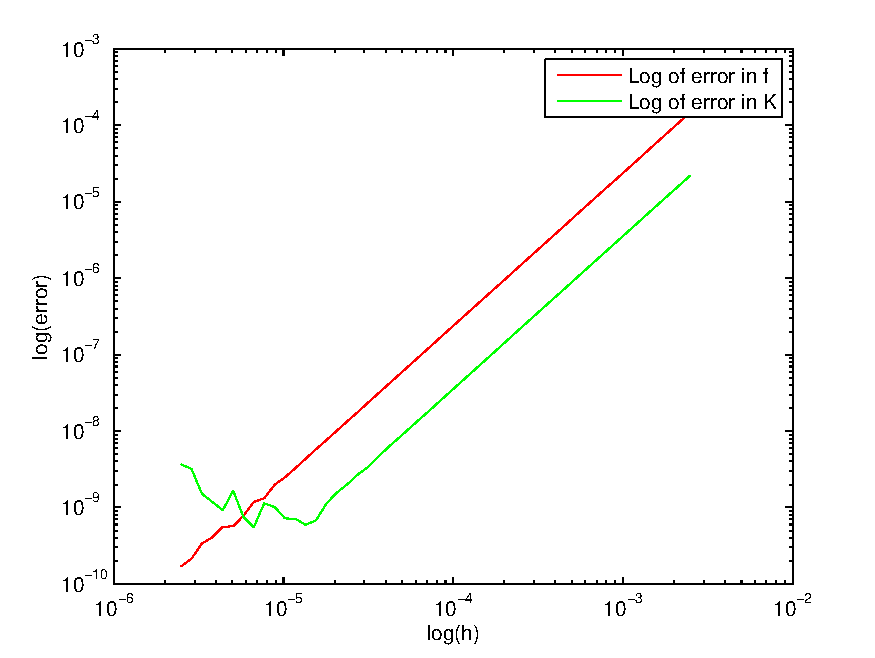
\includegraphics[scale=0.5]{./img/ConsistencyT3Lin.pdf}
    \caption{Linear 3-node triangular element}
    \label{fig:linCon}
  \end{subfigure}%
  \begin{subfigure}[b]{0.5\textwidth}
    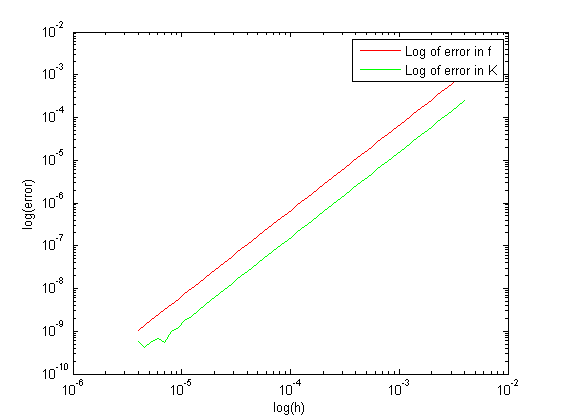
\includegraphics[scale=0.5]{./img/T6quadEleConsistency.png}
    \caption{Quadratic 6-node triangular element}
    \label{fig:quadCon}
  \end{subfigure}
  \caption{Log-log plot of error versus $h$ shows straight lines with
    slope 2 indicating error of $\mathcal{O}(h^2)$ as expected for a
    central finite difference numerical differentiation. Smaller vlues
    of $h$ introduce large rounding errors as seen in Figure
    ~\ref{fig:linCon}}
  \label{fig:consistency}
\end{figure}
\subsubsection*{Rank of Stiffness Matrix}
The fourth order stiffness modulus $K_{iakb}$ can be \textit{unrolled}
into a square 2-D matrix of size $ia\times kb$. For linear 3-node
triangular element this will give a $6\times6$ matrix and for the
quadratic 6-node triangular element we get a $12\times12$ matrix. A
$n\times n$ matrix can have maximum of $n$ non-zero eigenvalues. Then
the \textit{rank} of that matrix is said to be $n$. Each zero
eigenvalue reduces the rank by $1$ which makes the matrix \textit{rank
  deficient}. We calculated the rank of the stiffness matrix for the
case of zero deformation i.e. $\mathbf{X}=\mathbf{x}$ and for finite
deformation for different combinations of shape function and
quadrature order choices. The results are presented in Table
~\ref{tab:rank}. A discrete finite-element model must give unique
solution in the same way as the corresponding continuous mathematical
model. In a elasticity problem, rigid body motions do not result in
any internal forces and thus are called zero-energy modes. Zero-energy
modes make the solution degenerate i.e. non-unique. Each zero
eigen-value of the stiffness matrix should represents a rigid-body
mode and we should not have any extra zero-energy modes in our finite
element implementation than as physically expected. For zero
deformation case, there are three degrees of freedom --- two
translations and one rotation. Hence, we expect the stiffness matrix
to be rank-deficient by 3. For finite deformation case there are only
two degrees of freedom --- the translations. Hence, we expect the
matrix to be rank deficient by 2.
\begin{table}
  \centering
  \caption{Rank of stiffness matrix for various combinations of shape functions and order of Gaussian quadrature}
  \label{tab:rank}
  \begin{tabular}{|c|c|c|c|}
    \hline
    Deformation & Shape Function & Quadrature & Rank \\
    \hline
    \multirow{3}{*}{Zero} & Linear & 1-point & 3 \\
    \cline{2-4}
                & Quadratic & 1-point & 3 \\
    \cline{2-4}
                & Quadratic & 3-point & 9 \\
    \hline
    \multirow{3}{*}{Finite} & Linear & 1-point & 4 \\
    \cline{2-4}
                & Quadratic & 1-point & 4 \\
    \cline{2-4}
                & Quadratic & 3-point & 10 \\
    \hline
  \end{tabular}
\end{table}
The results presented in Table ~\ref{tab:rank} are consistent with our
expectations for all but the two cases when we use 1-point Gaussian
quadrature rule with a quadratic shape function. A 1-point Gaussian
quadrature rule can exactly reproduce an integration of a polynomial
of degree less than or equal to $1$. For exactly reproducing
integration of quadratic shape function we will need at least 3-point
quadrature. By using lesser number of sampling points we are
introducing extra non-physical zero body modes.
\section*{Source Code Listing}
The source code files for this assignment are listed below.
\begin{enumerate}
\item \texttt{aspectRation.m}:This function takes coordinates of
  vertices of a triangle as input and returns its aspect ratio as an
  output. We use it to ensure that we do not generate skewed triangles
  which can cause problems due determinant of $F$ approaching zero.
\item \texttt{checkOutwardNormal.m}: This function takes coordinates
  of vertices of a triangle as an input and checks if the sequence of
  the vertices is consistent with the node numbering of the standard
  parametric triangle. This is used to ensure that we don't get
  deformation gradients with negative determinant.
\item \texttt{findStiffnessRank.m}: This function accepts a four
  dimensional array as an input and unrolls it into a 2D matrix and
  returns the number of non-zero eigenvalues of the unrolled matrix as
  output.
\item \texttt{neoHookean.m} This is the 3D neo-Hookean constitutive
  model implementation from HW 1.
\item \texttt{planeStressNH.m} This is the plane-stress implementation
  of the 3D neo-Hookean consitutive model as developed for HW 1.
\item \texttt{Stiffness\_rank.m} This is a script file that calculates
  and prints a table for the rank of stiffness matrix for different
  combination of shape function and quadrature rule choices.
\item \texttt{T3Lin.m} This function takes $(r,s)$ coordinates as
  input and returns the shape function and its derivatives evaluated
  for a linear 3-node triangular element at that point.
\item \texttt{T6quad.m} This function takes $(r,s)$ coordinates as
  input and returns the shape function and its derivatives evaluated
  for a quadratic 6-node triangular element at that point.
\item \texttt{T3Lin\_Verification.m} This script runs the various tests
  for the linear 3-node shape functions.
\item \texttt{T6quad\_Verification.m} This script runs the various tests
  for the quadratic 6-node shape functions.
\item \texttt{T3LinEle.m} This function takes $X,x$, quadrature order
  and the material properties $\mu$ and $\lambda$ as input and returns
  the strain energy, internal force and stiffness modulus for a linear
  3-node triangular finite element.
\item \texttt{T6QuadEle.m} This function takes $X,x$, quadrature order
  and the material properties $\mu$ and $\lambda$ as input and returns
  the strain energy, internal force and stiffness modulus for a quadratic
  6-node triangular finite element.
\item \texttt{T3LinEle\_Verification.m}: This script runs and prints
  the results of various tests for the linear 3-node triangular
  element.
\item \texttt{T6QuadEle\_Verification.m}: This script runs and prints
  the results of various tests for the quadratic 6-node triangular
  element.
\item \texttt{TriGaussQuad.m}: This function takes the order of
  Gaussian quadrature as input and returns the corresponding sampling
  points and weights as output for a standard triangular domain.
\item \texttt{TriGaussQuad\_Verification.m}: This script runs
  verification test for the Gaussian quadrature implementation and
  prints its results.
\end{enumerate}
\end{document}

%%% Local Variables:
%%% mode: latex
%%% TeX-master: "../main"
%%% End:
